\PassOptionsToPackage{table}{xcolor}
\documentclass[t]{beamer}

\usepackage[T1]{fontenc}
\usepackage[utf8]{inputenc}
\usepackage[brazil]{babel}
\usepackage[round,authoryear]{natbib}
\usepackage{tabulary}
\usepackage{multicol}
\usepackage[table]{xcolor}

%%%% TEMAS %%%%
%\usetheme{Antibes}
%\usetheme{Bergen}
%\usetheme{Berkeley}
\usetheme{Berlin}
%\usetheme{Copenhagen}
%\usetheme{Darmstadt}
%\usetheme{Dresden}
%\usetheme{Frankfurt}
%\usetheme{Goettingen}
%\usetheme{Hannover}
%\usetheme{Ilmenau}
%\usetheme{JuanLesPins}
%\usetheme{Luebeck}
%\usetheme{Madrid}
%\usetheme{Malmoe}
%\usetheme{Marburg}
%\usetheme{Montpellier}
%\usetheme{PaloAlto}
%\usetheme{Pittsburgh}
%\usetheme{Rochester}
%\usetheme{Singapore}
%\usetheme{Szeged}
%\usetheme{Warsaw}
%\usetheme{boxes}
%\usetheme{default}
%\usetheme{CambridgeUS}

%%%% CORES %%%%

%\usecolortheme{default}
%\usecolortheme{albatross}
%\usecolortheme{beaver}
%\usecolortheme{beetle}
%\usecolortheme{crane}
%\usecolortheme{dolphin}
%\usecolortheme{dove}
%\usecolortheme{fly}
%\usecolortheme{lily}
%\usecolortheme{orchid}
%\usecolortheme{rose}
%\usecolortheme{seagull}
%\usecolortheme{seahorse}
%\usecolortheme{whale}
%\usecolortheme{wolverine}

%%%% TITULO %%%%
\title % (optional, only for long titles)
{Uma solução de aprendizagem de máquina para detecção de anomalias em imagens aéreas da floresta amazônica}
%\subtitle{Evidence from India}
\author %[Author, Anders] % (optional, for multiple authors)
{Candidato: Luiz Carlos A. M. Cavalcanti
\\Orientadora: Dr$^a$ Eulanda Miranda dos Santos} %\inst{1}}
%\institute[Universities Here and There] % (optional)
%{
%  \inst{1}%
%  Institute of Computer Science\\
%  University Here
%  \and
%  \inst{2}%
%  Institute of Theoretical Philosophy\\
%  University There
%}
\date[] % (optional)
{Exame de qualificação}
\subject{Computer Science}

\AtBeginSection[]
{
  \begin{frame}
    \frametitle{Roteiro}
    \tableofcontents[currentsection]
  \end{frame}
}

\begin{document}
  \begin{frame}\titlepage\end{frame}

%%%%%%%%%%%%%%%

\section{Contextualização}

\begin{frame}
\frametitle{Introdução}

	Amazônia legal:
	\begin{itemize}
		\item 11 mil km de fronteiras;
		\item 22 mil km de vias fluviais;
		\item 66\% do território nacional.
	\end{itemize}

	\vspace{0.5cm}

	Veículos Aéreos Não-Tripulados (VANTs) podem ser utilizados:
	\begin{itemize}
		\item Maior cobertura de área;
		\item Aproximação discreta;
		\item Variedade de sensores embarcados.
	\end{itemize}

\end{frame}

\begin{frame}
\frametitle{Motivação}

A quantidade maciça de dados gerados pelos VANTs leva à necessidade de desenvolvimento de procedimentos capazes de avaliar essa grande quantidade de material e identificar os prováveis objetos de interesse.

\begin{itemize}
	\item Maior rapidez na análise de dados;
	\item Redução da quantidade de informação a analizar;
	\item Necessidade de menos especialistas por missão.
\end{itemize}

Objetos de interesse:
\begin{itemize}
	\item Veículos terrestres e navais;
	\item Acampamentos, construções;
	\item Clareiras, pistas de pouso, estradas.
\end{itemize}


%Técnicas de PDI e AM podem ajudar a encontrar:

\end{frame}

\begin{frame}
\frametitle{Objetivos}

Geral:

\begin{itemize}
	\item Solução computacional que envolva PDI e AM para detecção de anomalias em imagens aéreas de floresta amazônica.
\end{itemize}

Específicos:

\begin{itemize}
    \item Organizar uma base de dados de imagens devidamente rotuladas que sirva de referência para futuros estudos desta problemática.
    \item Investigar e definir métodos para extração e seleção de características mais adequadas ao problema em questão.
    \item Realizar experimentos e apontar o melhor conjunto de técnicas para a detecção de anomalias em imagens aéreas da floresta amazônica.
\end{itemize}

\end{frame}

%%%%%%%%%%%%%%%

\section{Trabalhos relacionados}

\begin{frame}
	\frametitle{Trabalhos relacionados}
	
	O trabalho se propõe a utilizar técnicas de PDI e AM, portanto o levantamento bibliográfico foi dividido entre essas duas áreas de pesquisa, com os temas centrais:
	
	\vspace{0.5cm}
	
	\begin{itemize}
		\item Segmentação de imagens;
		\item Classificação de imagens aéreas.
	\end{itemize}
	
\end{frame}

\begin{frame}
	\frametitle{Trabalhos relacionados: Segmentação de imagens}
	
	\textbf{\textit{Berkeley Segmentation Dataset 500} (BSD500)}
	
	\vspace{.5cm}
		
	Conjunto de 500 imagens naturais. Todas as imagens possuem \textit{ground truth} de segmentação por seres humanos.
	
	\vspace{.5cm}
	
	Considerada uma das mais importantes bases de imagens naturais para comparação entre algoritmos de segmentação.

\end{frame}

\begin{frame}
	\frametitle{Trabalhos relacionados: Segmentação de imagens}

	\textbf{Systematic benchmarking of aerial image segmentation}
	
	\textit{Yuan, Gleason e Cheriyadat (2013)}
	
	\vspace{.5cm}
	
	Revisão dos algoritmos mais bem sucedidos na BSD500, utilizando uma nova base de imagens, composta apenas de imagens aéreas.
	
	\small{
	\begin{table}[h]
	\centering
	\begin{tabulary}{\linewidth}{|L|L|C|C|}
	\hline
	\textbf{Técnica} & \textbf{Características} & \textbf{Prec. bordas} & \textbf{Prec. regiões } \\ \hline
	Manual      & \hspace{1cm} -    & 69\% & 84\% \\ \hline
	gPb-owt-ucm & Cor, borda       & 65\% & 69\% \\ \hline
	FSEG        & Textura          & 61\% & 66\% \\ \hline
	SRM         & Cor, intensidade & 60\% & 60\% \\ \hline
	JSEG        & Cor, borda       & 56\% & 66\% \\ \hline
	MSEG        & Cor, morfologia  & 57\% & 50\% \\ \hline
	Mean-shift  & Cor, posição     & 58\% & 48\% \\ \hline
	\end{tabulary}
	\end{table}
	}

\end{frame}

%\begin{frame}
%	\frametitle{Trabalhos relacionados: Segmentação de imagens}
%
%	\textbf{Unsupervised segmentation of color-texture regions in images and video}
%
%	\textit{Deng e Manjunath (2001)}
%
%	\vspace{.5cm}
%
%	Apresenta o algoritmo JSEG, que segmenta a imagem em duas etapas:
%	\begin{enumerate}
%		\item Quantização das cores em diversas classes;
%		\item Computação da intensidade das bordas ($J$) a partir das cores quantizadas.
%	\end{enumerate}
%
%	\vspace{.5cm}
%
%	As regiões são obtidas a partir de crescimento de região com base no valor de $J$.
%
%\end{frame}
%
%\begin{frame}
%	\frametitle{Trabalhos relacionados: Segmentação de imagens}
%	\textbf{Mean shift: a robust approach toward feature space analysis}
%
%	\textit{Comaniciu e Meer (2002)}
%
%	\vspace{0.5cm}
%
%	O algoritmo computa vetores de mean-shift iterativamente para mapear pixels para o domínio espacial e de cores do centro de seus \textit{clusters}. Após a convergência, os \textit{clusters} são fundidos de acordo com parâmetros de similaridade. 
%
%	\vspace{0.5cm}
%
%	Parâmetros como largura de banda espacial, de cores e o tamanho do menor \textit{cluster} podem ser utilizados para adequar o algoritmo ao problema em questão.
%
%
%\end{frame}
%
%\begin{frame}
%	\frametitle{Trabalhos relacionados: Segmentação de imagens}
%
%	\textbf{Efficient graph-based image segmentation}
%
%	\textit{Felzenszwalb e Huttenlocher (2004)}
%
%	\vspace{0.5cm}
%
%	O algoritmo MSEG é amplamente usado pela comunidade de sensoriamento remoto.
%
%	\vspace{0.5cm}
%
%	Sob a óptica de grafos, os pixels são tratados como nodos e os pesos de suas arestas representam a diferença entre características entre os pixels. Um segmento corresponde a um componente conectado.
%\end{frame}
%
%\begin{frame}
%	\frametitle{Trabalhos relacionados: Segmentação de imagens}
%
%	\textbf{Statistical region merging}
%
%	\textit{Nock e Nielsen (2004)}
%
%	\vspace{0.5cm}
%
%	O algoritmo SRM utiliza um procedimento simples de junção acompanhado por uma operação de ordenação para segmentar imagens com eficiência. Duas regiões são unidas se a diferença entre os valores médios dos pixels das duas regiões estão abaixo de um limiar. 
%
%	\vspace{0.5cm}
%
%	A coesão da segmentação pode ser controlada por um parâmetro definido pelo usuário.
%
%\end{frame}
%
%\begin{frame}
%	\frametitle{Trabalhos relacionados: Segmentação de imagens}
%
%	\textbf{Contour Detection and Hierarchical Image Segmentation}
%
%	\textit{Arbelaez et al. (2011)}
%
%	\vspace{0.5cm}
%
%	O algoritmo gPb-owt-ucm realiza segmentação em várias etapas. Primeiramente a técnica combina informações de intensidade, textura e coloração para computar vetores que servirão como detectores de contorno. Posteriormente, uma técnica de \textit{watershed} é aplicada à saída do detector de contornos para produzir uma segmentação hierárquica da imagem.
%
%\end{frame}
%
%\begin{frame}
%	\frametitle{Trabalhos relacionados: Segmentação de imagens}
%
%	\textbf{Factorization-based texture segmentation}
%
%	\textit{Yuan e Wang (2013)}
%
%	\vspace{0.5cm}
%
%	O FSEG primeiramente computa o histograma espectral para cada pixel da imagem. A proposta é que cada característica pode ser aproximada por uma combinação linear de diversas características representativas e suas combinações ponderadas. 
%
%	\vspace{0.5cm}
%
%	Por fim, um pixel é dito pertencente à região com maior peso. O algoritmo FSEG utiliza decomposição de valores singulares e fatoração de matrizes não-negativas para aumentar a eficiência computacional da segmentação.
%
%\end{frame}
%
%\begin{frame}
%	\frametitle{Trabalhos relacionados: Segmentação de imagens}
%
%	Resultados em \textbf{Yuan, Gleason e Cheriyadat (2013)}:
%
%	\small{
%	\begin{table}[h]
%	\centering
%	\begin{tabulary}{\linewidth}{|L|L|C|C|}
%	\hline
%	\textbf{Técnica} & \textbf{Características} & \textbf{Prec. bordas} & \textbf{Prec. regiões } \\ \hline
%	Manual      & \hspace{1cm} -    & 69\% & 84\% \\ \hline
%	gPb-owt-ucm & Cor, borda       & 65\% & 69\% \\ \hline
%	FSEG        & Textura          & 61\% & 66\% \\ \hline
%	SRM         & Cor, intensidade & 60\% & 60\% \\ \hline
%	JSEG        & Cor, borda       & 56\% & 66\% \\ \hline
%	MSEG        & Cor, morfologia  & 57\% & 50\% \\ \hline
%	Mean-shift  & Cor, posição     & 58\% & 48\% \\ \hline
%	\end{tabulary}
%	\end{table}
%	}
%
%\end{frame}

\begin{frame}
	\frametitle{Trabalhos relacionados: Classificação de imagens aéreas}

	Os trabalhos levantados acerca desta seção tratam de classificação de imagens aéreas para fins de mapeamento ou detecção de características específicas. 
	
	\vspace{0.5cm}

	Os trabalhos foram selecionados por estar de acordo com as seguintes características das imagens utilizadas:

	\begin{itemize}
		\item Altitude entre 1000 e 5000 metros;
		\item Inclinação de aproximadamente 90\%;
		\item Imagens com forte presença de vegetação.
	\end{itemize}

%\end{frame}

%\begin{frame}
%	\frametitle{Trabalhos relacionados: Classificação de imagens aéreas}
%
%	\textbf{Color and texture fusion: application to aerial image segmentation and GIS updating}
%
%	\textit{Dubuisson-Jolly e Gupta (2000)}
%
%	\vspace{0.5cm}
%
%	Apresenta uma técnica de segmentação focada em imagens aéreas coloridas que realiza a segmentações separadamente por cor e textura, para no final unir as duas e chegar a uma segmentação final utilizando um algoritmo de classificação por \textit{Maximum Likelihood}.
%
%\end{frame}
%
%\begin{frame}
%	\frametitle{Trabalhos relacionados: Classificação de imagens aéreas}
%
%	\textbf{Aerial image processing and object recognition}
%
%	\textit{Sadgal, Fazziki e Ouahman (2005)}
%
%	\vspace{0.5cm}
%
%	Sugere pré-processamento, segmentação e reconhecimento em uma única etapa. Combina métodos estocásticos (inferência Bayesiana, campos de Markov) e não-estocásticos (redes neurais).
%
%	\vspace{0.5cm}
%
%	Métodos são unidos no final do processo, permitindo parelelização de boa parte da solução.
%
%\end{frame}
%
%\begin{frame}
%	\frametitle{Trabalhos relacionados: Classificação de imagens aéreas}
%
%	\textbf{A simple and efficient method for segmentation and classification of aerial images}
%
%	\textit{Ahmadi (2013)}
%
%	\vspace{0.5cm}
%
%	Utiliza características de cor (HSV) e textura (filtro de Gabor) e KNN para  realizar classificação de tipos de terreno em imagens aéreas.
%
%\end{frame}
%
%\begin{frame}
%	\frametitle{Trabalhos relacionados: Classificação de imagens aéreas}
%
%	\textbf{Fast semantic segmentation of aerial images based on color and texture}
%
%	\textit{Ghiasi e Amirfattahi (2013)}
%
%	\vspace{0.5cm}
%
%	Realiza segmentação e classificação de tipos de terreno em imagens aéreas.
%
%	\vspace{0.5cm}
%
%	A imagem é dividida em superpixels (fluxos geométricos de Levishtein) e características de cor (RGB) e textura (LBP-HF) são extraídas. Cada superpixel é classificado com KNN.
%
\end{frame}

\begin{frame}[c]
	\frametitle{Trabalhos relacionados: Classificação de imagens aéreas}
	\small{
		\begin{table}[h]
		\centering
		\begin{tabulary}{\linewidth}{|L|L|L|L|C|}
		\hline
		\textbf{Trabalho} &  \textbf{Aprendizado} & \textbf{Problema investigado} &  \textbf{Precisão} \\ \hline
		Dub-Jolly & Máxima veross. & Atualização de mapas           & 91,86\% \\ \hline
		Sadgal    & Redes neurais          & Classificação de terreno       & -       \\ \hline
		Ahmadi    & KNN                    & Classificação de terreno       & 82,23\% \\ \hline
		Ghiasi    & KNN                    & Busca por objetos & 95\%    \\ \hline
		\end{tabulary}
		\end{table}
	}
\end{frame}

%%%%%%%%%%%%%%%

\section{Metodologia}

\begin{frame}[c]
	\frametitle{Metodologia}
	\begin{figure}[h]
    	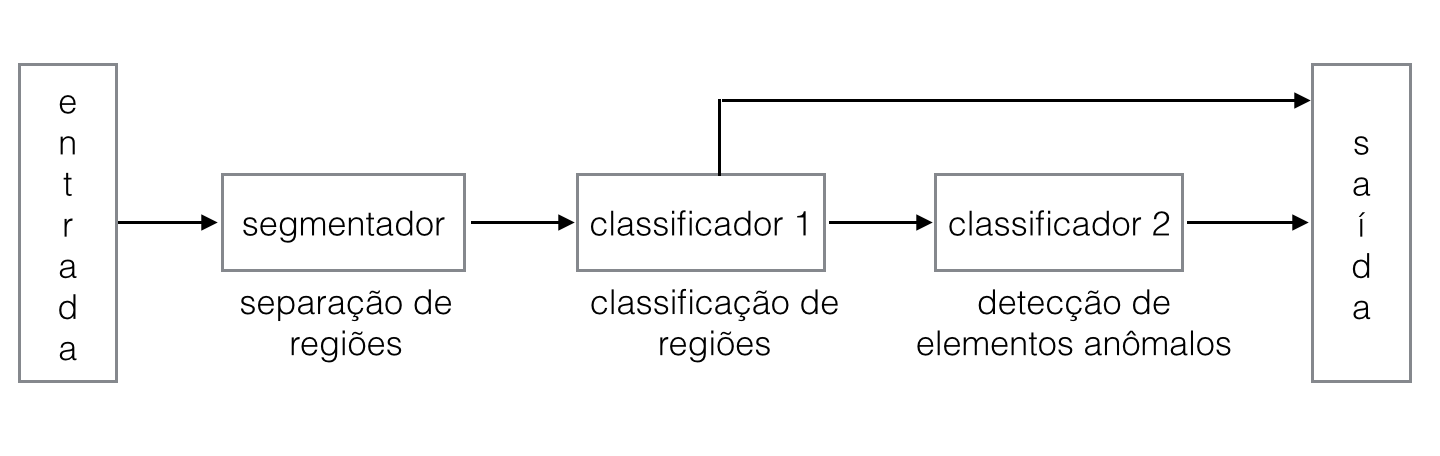
\includegraphics[width=\textwidth]{imgs/arquitetura}
	\end{figure}
\end{frame}

\begin{frame}[c]
	\frametitle{Metodologia: Segmentação}
	\begin{figure}[h]
    	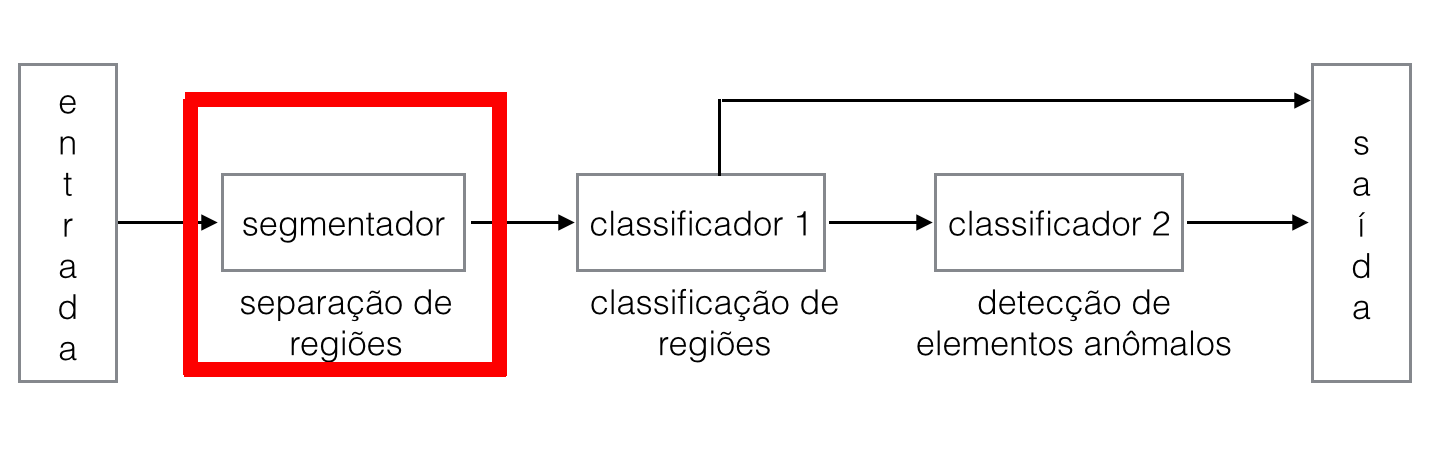
\includegraphics[width=\textwidth]{imgs/arquitetura_1}
	\end{figure}
\end{frame}

\begin{frame}
	\frametitle{Metodologia: Segmentação}

	A primeira etapa do trabalho é a segmentação das imagens por tipo de terreno. Uma porção da base de imagens será manualmente segmentada por seres humanos e servirá de base de comparação para a segmentação realizada pelos métodos experimentados.

	\begin{multicols}{2}
		\begin{figure}
			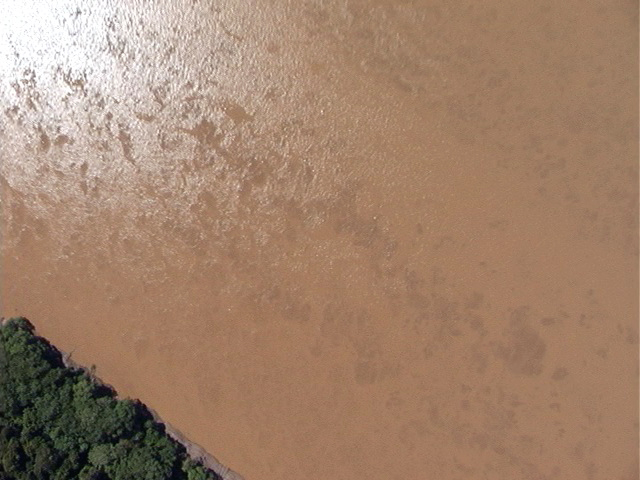
\includegraphics[scale=0.4]{imgs/exemplo_segmentacao}
		\end{figure}
		\begin{figure}
			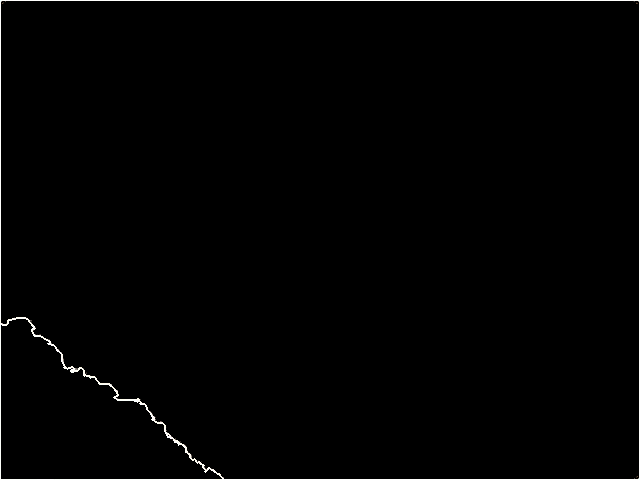
\includegraphics[scale=0.2]{imgs/exemplo_segmentacao2}
		\end{figure}
	\end{multicols}

\end{frame}

\begin{frame}[c]
	\frametitle{Metodologia: Primeira classificação}
	\begin{figure}[h]
    	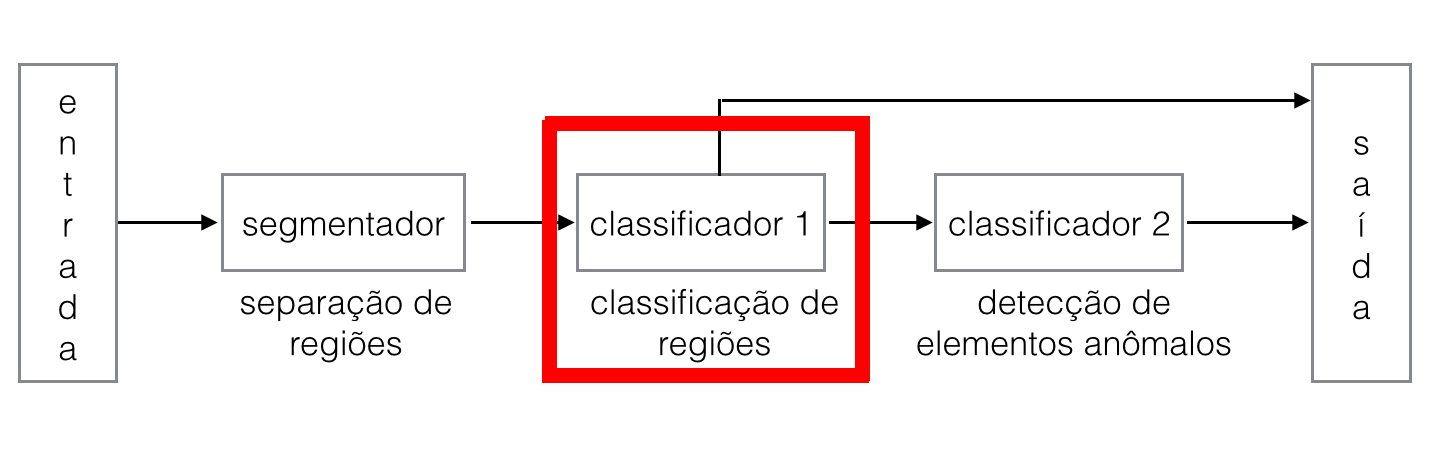
\includegraphics[width=\textwidth]{imgs/arquitetura_2}
	\end{figure}
\end{frame}

\begin{frame}
	\frametitle{Metodologia: Primeira classificação}

	As regiões encontradas na fase de segmentação são rotuladas por tipo de terreno:

	\begin{itemize}
		\item Floresta;
		\item Vegetação rasteira;
		\item Clareira/descampado;
		\item Água;
		\item Elementos anômalos.
	\end{itemize}

	Regiões rotuladas como "elementos anômalos" são consideradas regiões de interesse. As demais serão inspecionadas em uma segunda etapa de classificação. Os resultados de cada método serão comparados à uma classificação realizada por seres humanos.

\end{frame}

\begin{frame}[c]
	\frametitle{Metodologia: Segunda classificação}
	\begin{figure}[h]
    	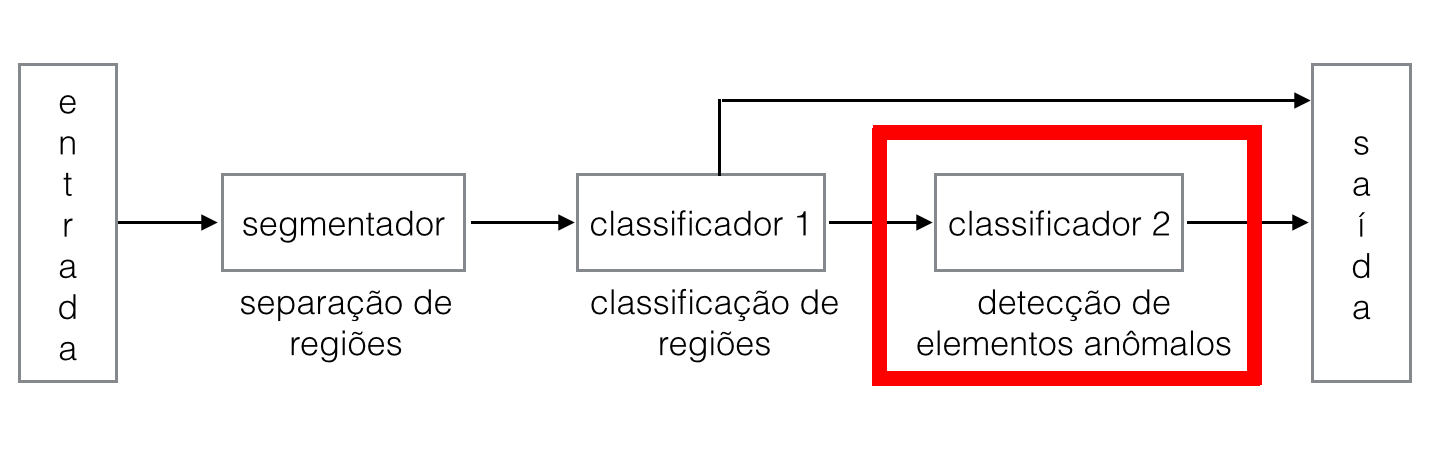
\includegraphics[width=\textwidth]{imgs/arquitetura_3}
	\end{figure}
\end{frame}

\begin{frame}
	\frametitle{Metodologia: Segunda classificação}

	A última etapa de classificação consiste em utilizar modelos de aprendizado específicos para cada tipo de terreno, para detectar objetos de interesse que não foram encontrados na etapa de segmentação, normalmente pequenos demais para serem definidos como uma região \textit{per se}, e que estão contidos em regiões maiores.

	\vspace{0.5cm} 

	Isso permite que cada tipo de terreno possa usar seus próprios métodos de aprendizado e características da imagem.

	\vspace{0.5cm}

	Nesta etapa serão explorados classificadores unários e multi-classe a fim de obter o melhor resultado na detecção dos objetos de interesse e um classificador, com seus parâmetros e vetor de características, será selecionado para cada tipo de terreno.
\end{frame}

\begin{frame}[c]
	\frametitle{Metodologia: Saída}
	\begin{figure}[h]
    	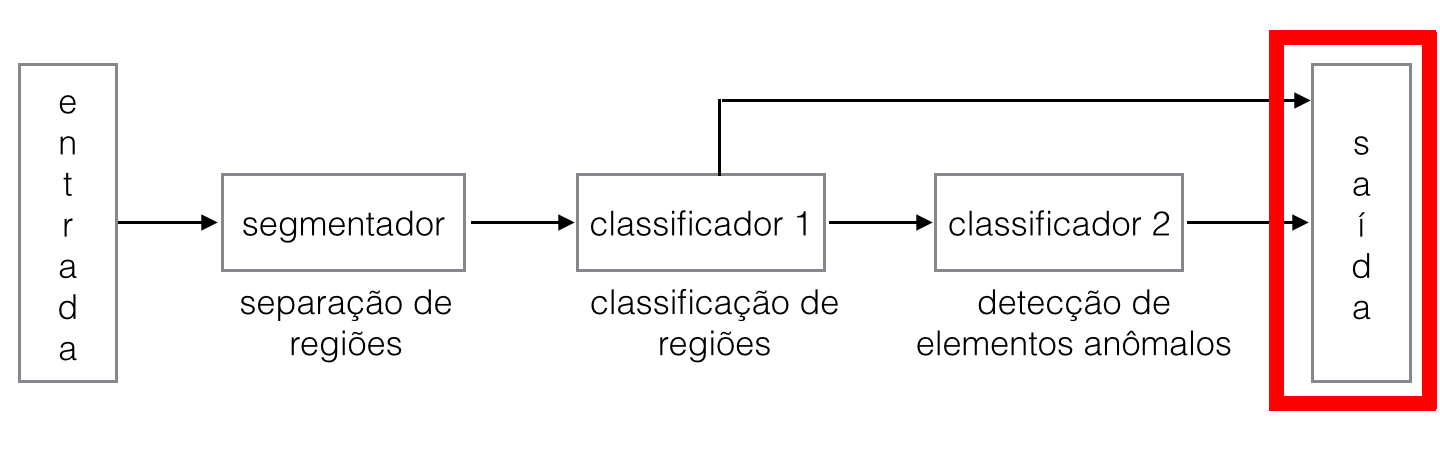
\includegraphics[width=\textwidth]{imgs/arquitetura_4}
	\end{figure}
\end{frame}

\begin{frame}
	\frametitle{Metodologia: Saída}

	Por fim, unindo a saída do primeiro nível de classificação, onde regiões de "elementos anômalos" podem ser encontradas, com a saída do segundo nível de classificação, onde os objetos de interesse serão procurados no interior das demais regiões, teremos uma saída única, apontando as regiões de uma imagem que possuam objetos de interesse na problemática em questão.

\end{frame}

%%%%%%%%%%%%%%%

\section{Resultados preliminares}

\begin{frame}
	\frametitle{Base de dados}

	\begin{itemize}
		\item 3.044 imagens em cores;
		\item Formato: JPEG;
		\item Dimensões: 640 x 480 pixels;
		\item 1,02 GB de dados.
	\end{itemize}

	\begin{multicols}{3}
		\begin{figure}
			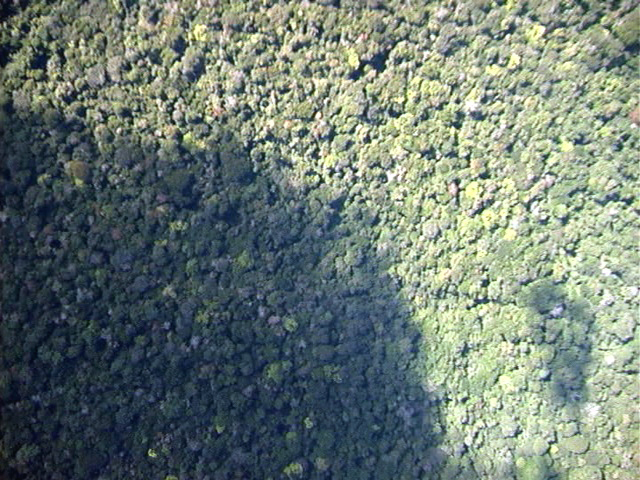
\includegraphics[scale=0.3]{imgs/amostra1}
		\end{figure}
		\begin{figure}
			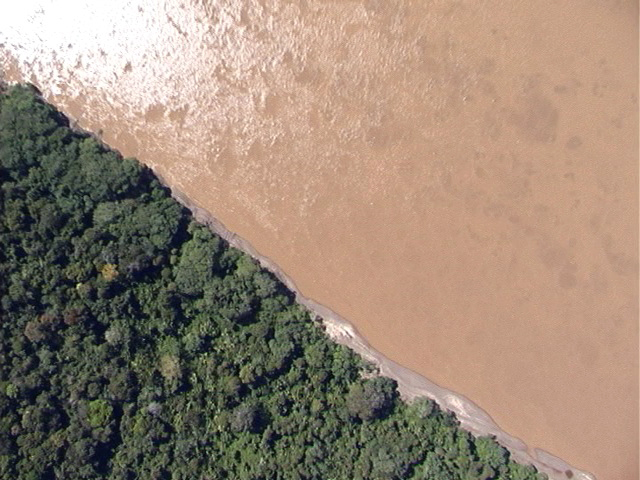
\includegraphics[scale=0.3]{imgs/amostra2}
		\end{figure}
		\begin{figure}
			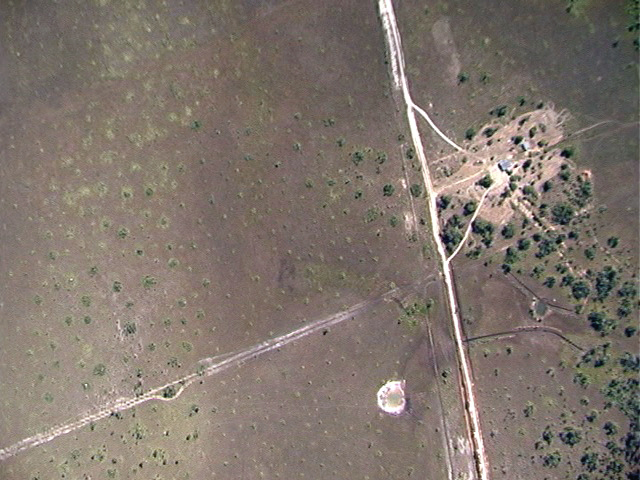
\includegraphics[scale=0.3]{imgs/amostra3}
		\end{figure}
	\end{multicols}

\end{frame}

\begin{frame}
	\frametitle{Base de dados}

	Uma ferramenta foi construída para segmentação e classificação da base de dados para as duas primeiras etapas do trabalho.

	\begin{figure}[h]
  		\centering
		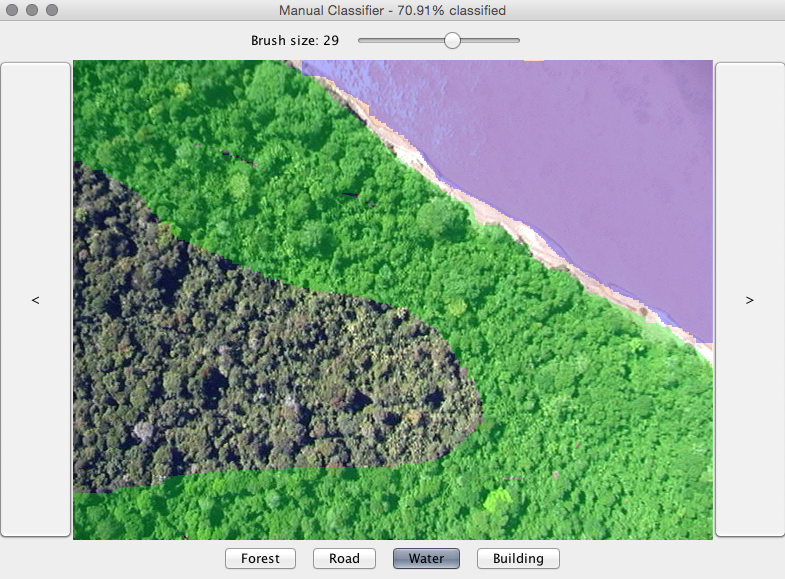
\includegraphics[scale=0.25]{imgs/visualClassifier}
	\end{figure}

\end{frame}

\begin{frame}
	\frametitle{Segmentação}

	\begin{itemize}
		\item 150 imagens;
		\item Medição de resultados por sobreposição e orientação de \textit{edgels} (Martin et al., 2001)
	\end{itemize}

	\small{
	\begin{table}
	\centering
	\begin{tabulary}{\linewidth}{|L|R|R|}
		\hline
		\textbf{Algoritmo} & \textbf{Acurácia} & \textbf{Tempo/imagem} \\ \hline
		Mean-shift  & 97,2\% & 6,39 s \\ \hline
		JSEG        & 96,3\% & 14,82 s \\ \hline
		MSEG        & 94,1\% & 0,33 s \\ \hline
		SRM         & 91,9\% & 4,66 s \\ \hline
		FSEG        & 81,4\% & 13,91 s \\ \hline
		gPb-owt-ucm & 72,2\% & 237,32 s \\ \hline
	\end{tabulary}
	\end{table}
	}

\end{frame}

\begin{frame}[c]
	\frametitle{Segmentação}

	\begin{figure}[c]
  		\centering
		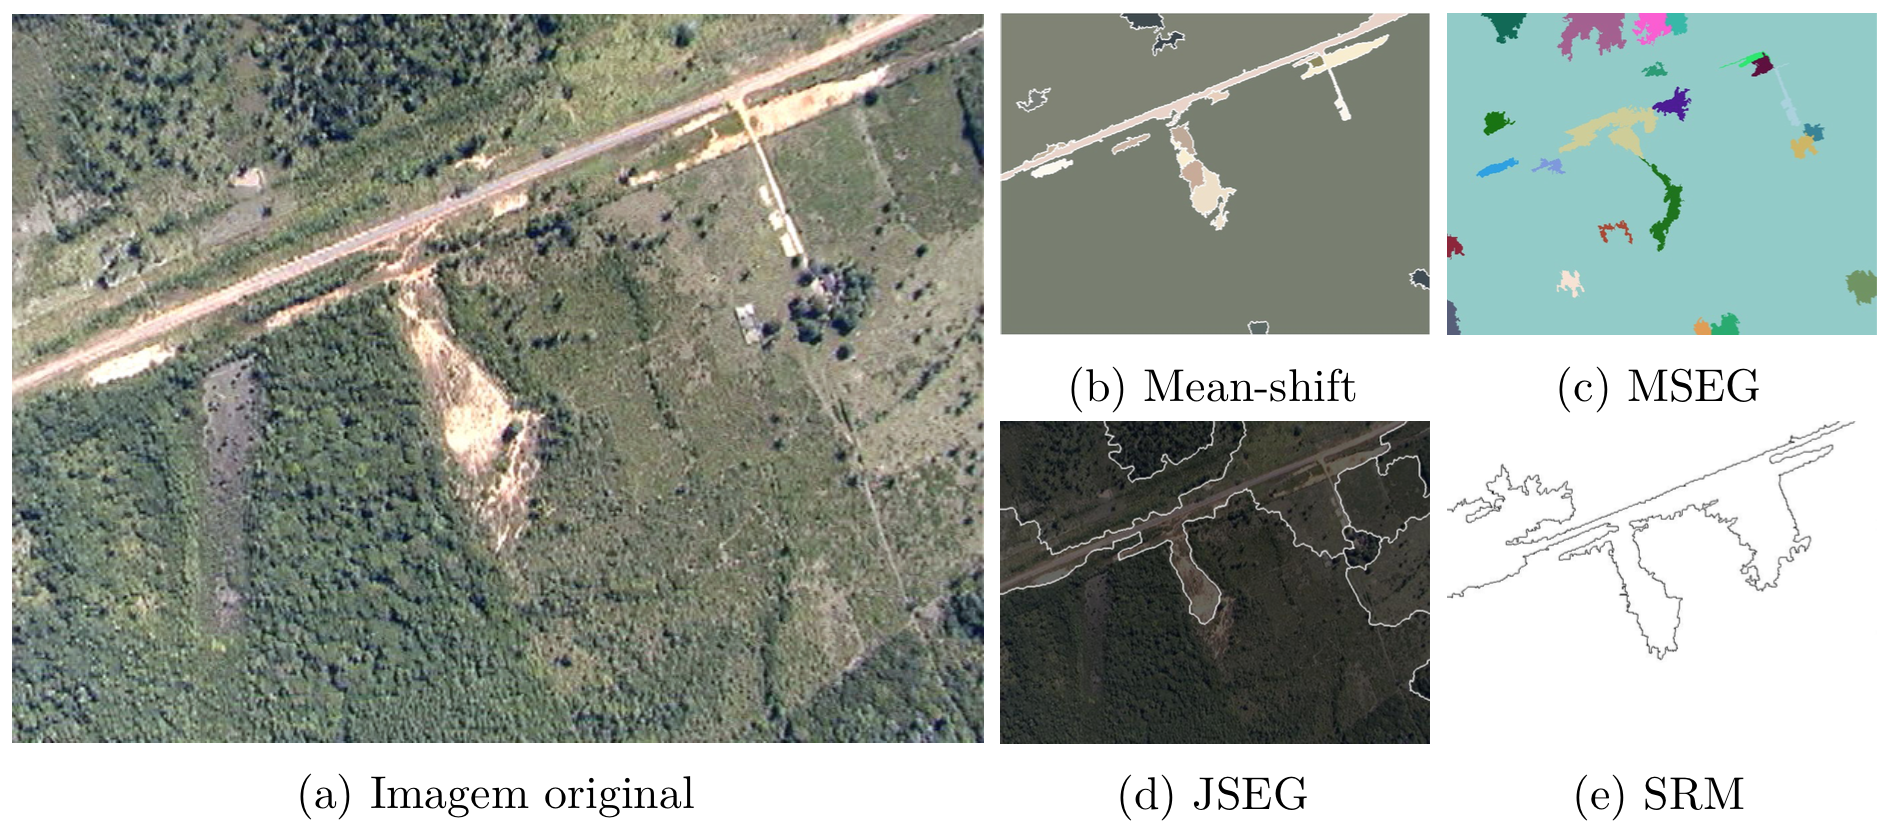
\includegraphics[width=\textwidth]{imgs/gambi_apresentacao}
	\end{figure}

\end{frame}

\begin{frame}[c]
	\frametitle{Segmentação}

	\begin{figure}[c]
		\centering
		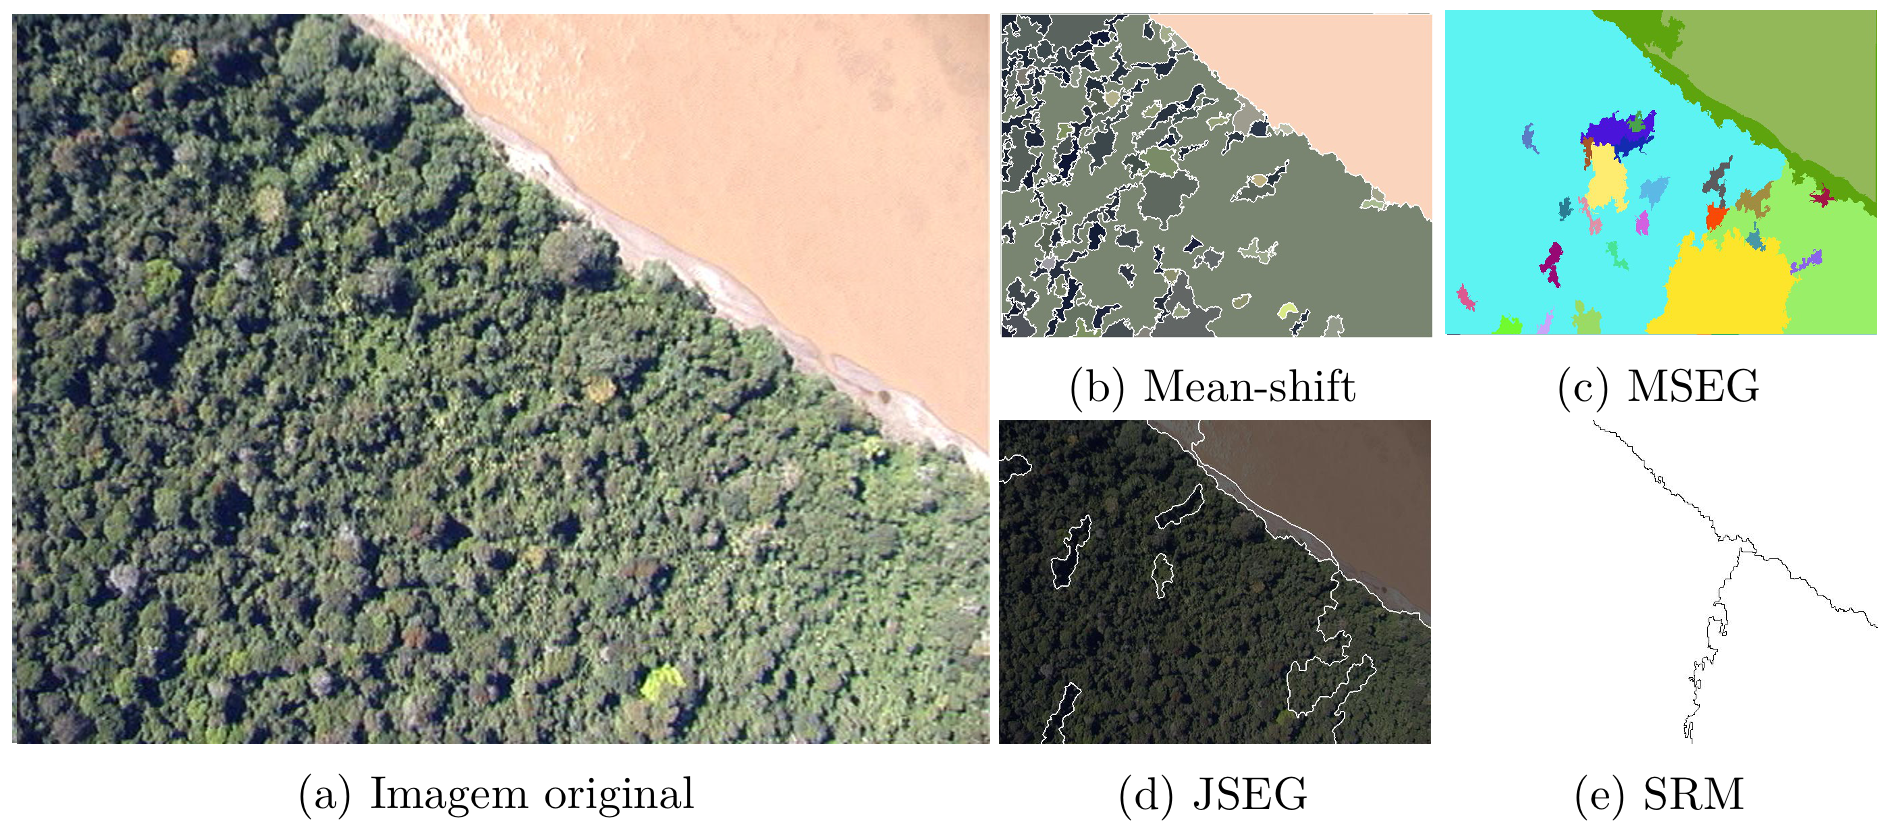
\includegraphics[width=\textwidth]{imgs/gambi_apresentacao2}
	\end{figure}

\end{frame}

\begin{frame}
	\frametitle{Segmentação}

	Um experimento para realizar segmentação e a primeira classificação em uma única etapa foi realizado, um artigo sobre o experimento foi publicado  na conferência VISAPP 2015. 

	\small{
	\begin{table}
	\centering
	\begin{tabulary}{\linewidth}{|L|R|R|}
		\hline
		\textbf{Algoritmo} & \textbf{Acurácia} & \textbf{Tempo/imagem} \\ \hline
		Random forest  & 96,0\% & 12,72 s \\ \hline
		KNN            & 92,6\% & 22,89 s \\ \hline
		Naive Bayes    & 92,8\% & 8,36 s \\ \hline
		Decision tree  & 82,2\% & 14,49 s \\ \hline
	\end{tabulary}
	\end{table}
	}

\end{frame}

\begin{frame}
	\frametitle{Primeira classificação}

	Características utilizadas:
	\begin{itemize}
		\item Cor média dos canais R, G e B;
		\item Histograma dos canais R, G e B;
		\item Grayscale médio;
		\item Histograma grayscale.
	\end{itemize}

%	\vspace{0.5cm}

%	Para o experimento, as mesmas 150 imagens usadas para segmentação foram utilizadas, resultando em 7.111 amostras (regiões segmentadas). Destas, 66\% serviram como amostras de treinamento e 33\% foram utilizadas como amostras de validação.

%\end{frame}

%\begin{frame}[c]
%	\frametitle{Primeira classificação}

	\small{
	\begin{table}[h]
	\centering
	\begin{tabulary}{\linewidth}{|L|R|R|R|}
		\hline
		\textbf{Método} & \textbf{Acurácia} & \textbf{Precisão} & \textbf{Revocação} \\ \hline
		SVM               & 89,19\% & 0,927 & 0,864 \\ \hline
		KNN               & 88,51\% & 0,912 & 0,863 \\ \hline
		Árvore de decisão & 87,09\% & 0,842 & 0,859 \\ \hline
	\end{tabulary}
	\end{table}
	}

\end{frame}

\begin{frame}
	\frametitle{Primeira classificação}

	\centering
	7.111 amostras (66\%/33\%).

	\small{
	\begin{table}[h]
	\centering
	\begin{tabulary}{\linewidth}{|L|R|R|}
		\hline
		\textbf{Classe} & \textbf{Amostras} & \textbf{Percentual} \\ \hline
		Floresta           & 4844 & 68,12\% \\ \hline
		Vegetação rasteira & 893  & 12,56\% \\ \hline
		Clareira           & 237  & 03,33\% \\ \hline
		Água               & 1123 & 15,79\% \\ \hline
		Elementos anômalos & 14   & 00,20\% \\ \hline
	\end{tabulary}
	\end{table}
	}

\end{frame}

\begin{frame}
	\frametitle{Próximos passos}

	\begin{itemize}
		\item Experimentar com ensembles de classificadores para a primeira classificação;
		\item Experimentar mais características para a primeira classificação: bordas, textura, morfologia, bag of visual words, vizinhança;
		\item Fazer levantamento de características para a segunda classificação;
		\item Realizar experimentos com classificadores unitários.
	\end{itemize}

\end{frame}
%%%%%%%%%%%%%%%

\section{Cronograma}

\begin{frame}[c]
	\frametitle{Cronograma}
	\begin{table}[h]
	\resizebox{\textwidth}{!}{%
	\begin{tabular}{|l|c|c|c|c|c|c|c|c|c|c|c|c|}
		\hline
		Atividade/Mês & 02/14 & 03/14 & 04/14 & 05/14 & 06/14 & 07/14 & 08/14 & 09/14 & 10/14 & 11/14 & 12/14 & 01/14 \\ \hline
		Disciplinas & \cellcolor{blue!25} & \cellcolor{blue!25} & \cellcolor{blue!25} & \cellcolor{blue!25} & \cellcolor{blue!25} & \cellcolor{blue!25} & \cellcolor{blue!25} & \cellcolor{blue!25} & \cellcolor{blue!25} & \cellcolor{blue!25} & \cellcolor{blue!25} & \cellcolor{blue!25} \\ \hline
		Levantamento &  &  &  & \cellcolor{blue!25} & \cellcolor{blue!25} & \cellcolor{blue!25} & \cellcolor{blue!25} &  &  &  &  &  \\ \hline
		Experimentos &  &  &  &  &  &  & \cellcolor{blue!25} & \cellcolor{blue!25} & \cellcolor{blue!25} & \cellcolor{blue!25} & \cellcolor{blue!25} & \cellcolor{blue!25} \\ \hline
	\end{tabular}
	}
	\end{table}

	\begin{table}[h]
	\resizebox{\textwidth}{!}{%
	\begin{tabular}{|l|c|c|c|c|c|c|c|c|c|c|c|c|}
		\hline
		Atividade/Mês & 02/15 & 03/15 & 04/15 & 05/15 & 06/15 & 07/15 & 08/15 & 09/15 & 10/15 & 11/15 & 12/15 & 01/16 \\ \hline
		Experimentos & \cellcolor{blue!25} & \cellcolor{blue!25} & \cellcolor{blue!25} & \cellcolor{blue!25} & \cellcolor{blue!25} & \cellcolor{blue!25} & \cellcolor{blue!25} & & & & & \\ \hline
		Sub. de artigos & & & & \cellcolor{blue!25} & \cellcolor{blue!25} & \cellcolor{blue!25} & \cellcolor{blue!25} &  &  &  &  &  \\ \hline
		Dissertação &  &  &  & \cellcolor{blue!25} & \cellcolor{blue!25} & \cellcolor{blue!25} & \cellcolor{blue!25} & \cellcolor{blue!25} & \cellcolor{blue!25} & \cellcolor{blue!25} & & \\ \hline
	\end{tabular}
	}
	\end{table}

\end{frame}

%\section{Bibliografia}

%\begin{frame}{Referências}
%	\tiny{\bibliographystyle{abbrv}}
%	\tiny{\bibliographystyle{apacite}}
%	\bibliographystyle{humannat}
%	\bibliography{qualificacao}
%\end{frame}

\end{document}